\chapter{Software architecture and implementation}
%Can put pseudocode in for main steps
%put the details of the examples in results and analysis chapter

\section{Simulator}\label{sec:sim}
%Pr 1 St 2
%software architechure
\subsection{Design objectives}

%Review design objectives
The primary objective of this work is to explore calibration, imaging and parameter estimation algorithms and systematic errors through synthetic data simulation. In order to address the many questions within the wide scope of this objective, one must be able to setup and run a diversity of experiments easily within the simulation framework. The major requirement which this puts on the architechure, is that it must be flexible and extendable.  

\subsection{Architechure and Work flow}

%overall architechure
In order to meet the design criteria, the simulator has been written in \textsc{Python} and {\sc MeqTrees} uses the {\sc measurement set}\footnote{https://casa.nrao.edu/Memos/229.html}  data format. \textsc{Python} is known for it's readability and has a wide user base in the astronomy community. The {\sc measurement set} is data format of choice as it is the provides direct access to data, although in the mm-VLBI field other formats are currently still more popular i.e. UVFITS or HOPS but with the rise of ALMA, the MS format will inevitably become the next generator data format and already is used at JIVE.


The primary outputs of the pipeline are an interferometric dataset in {\sc measurement set} format along with the closure phases and uncertainties and a dirty and/or cleaned image. The modular structure of the pipeline allows for multiple imaging and deconvolution algorithms to be employed. 
The highest level or driver script is written in Python which interfaces easily with other systems.  The bulk of the computational load is called through other programs, written in C++ which are faster. 

%back end


%front end

from source variability: To test these effects, we include time variability for source in meqs. A discussion of calibration and interpretation of time variability, including separating out time-variable and quiescent structure is outside the scope of this thesis, but hopefully mm-VLBI can use some techniques from other time-variable domains of interferometry like pulsar searches or scintillation analyses.

%work flow
A flow diagram of the simulator is shown in Fig.~\ref{flow}. Input to the simulator is a sky model and configuration file. The former is typically a time-ordered list of {\sc fits} images, where each image represents the source total intensity\footnote{Later versions of {\sc MeqSilhouette} will enable the full Stokes cubes as input.} over a time interval $\Delta t_{\rm src} = t_{\rm obs}/N_{\rm src}$, where $t_{\rm obs}$ is the observation length and $N_{\rm src}$ is the number of source images. The configuration file specifies all parameters needed by the pipeline to determine the particular observation configuration (array, frequency, bandwidth, start time, etc) and which signal corruption implementation should be employed.




\begin{figure*}
\begin{center}
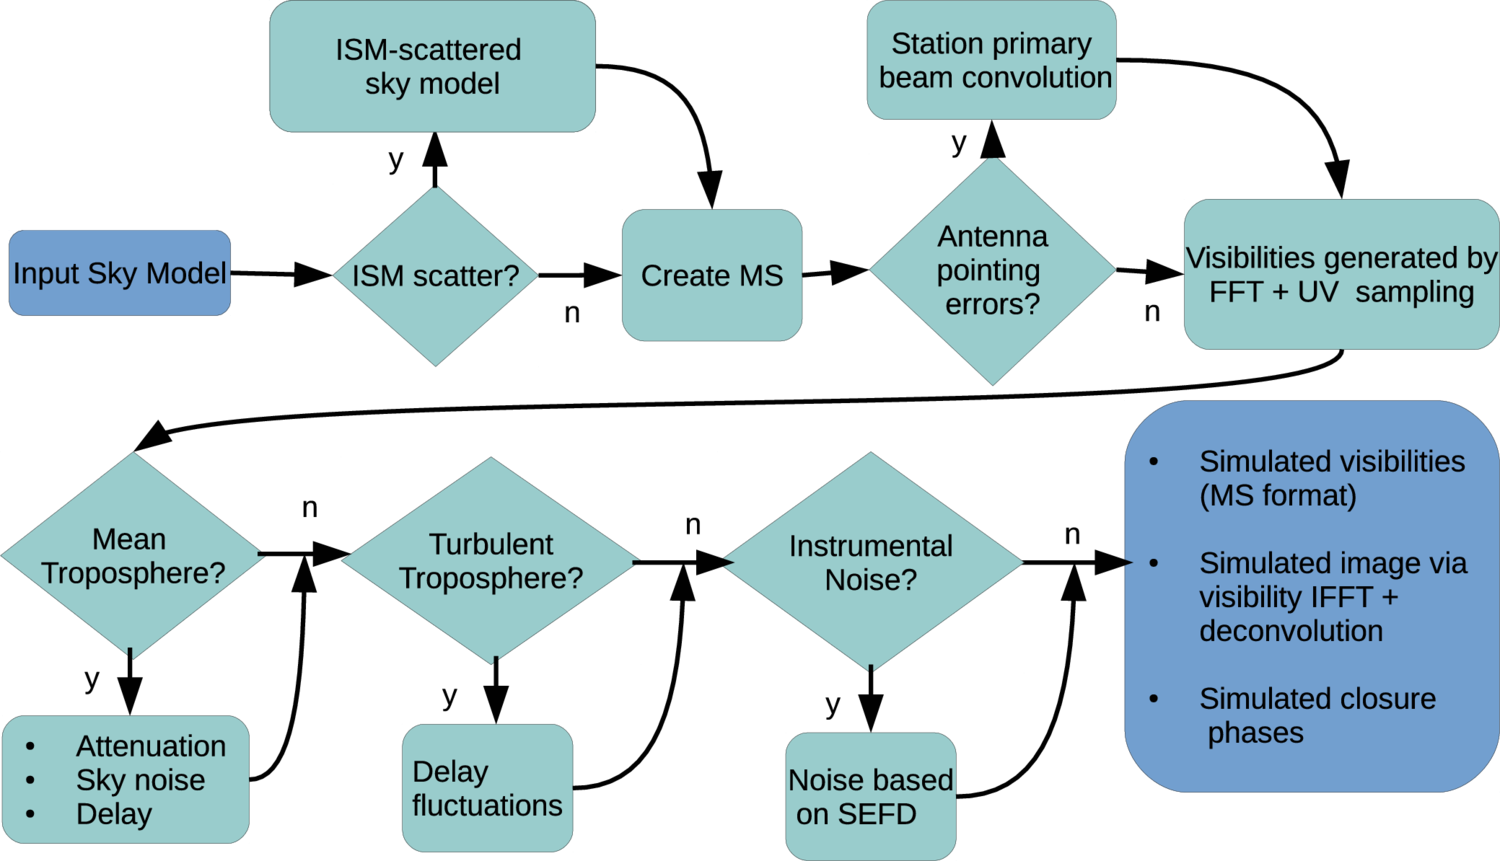
\includegraphics[width=\columnwidth]{Images/flow_full}
\caption{Flow diagram showing basic sequence of the \textsc{MeqSilhouette} simulation pipeline. The sky model could include (a) a time-ordered list of {\sc fits} images or (b) parametric source model consisting of Gaussians or point sources. The details of the station information, observation strategy, tropospheric and ISM conditions are specified in a user-defined input configuration file. The pipeline is flexible, allowing any additional, arbitrary Jones matrices to be incorporated. Further details in text.\label{flow}%
}
\end{center}
\end{figure*}


\subsection{ScatterBrane}
%Pr 1 St 2
%link back to theory
%Implementation in ScatterBrane : Python, the key algorithmic steps
%Integration of Scatterbrane
The turbulent phase screen $\phi(\mathbf{x})$ can generated from the phase spatial power spectrum (see Appendix C \citet*{Johnson_2015a}). 

Scattering in the ISM at millimetre wavelengths falls into the strong scattering regime, which has been quantitatively described in the literature \citep*{Narayan_1989,Goodman_1989} and implemented in the \textsc{Python}-based \textsc{Scatterbrane}\footnote{http://krosenfeld.github.io/scatterbrane/current} package, based on \citet*{Johnson_2015a}. This approach extends the turbulent model described in section~\ref{sec:basic_scat} to regimes where the inner and outer turbulent scales as well as the anisotropy of scattering kernel are considered. The distance to the screen is taken from the best-fit solution from \citet{Bower_2013} and is located, not at the Galactic Centre, but rather in the Scutum spiral arm at a distance $D_{\rm os}=5.8 \pm 0.3$~kpc. 


We aim to place this description of ISM scattering, which has already yielded an important context for mm-VLBI observation \citep[e.g.][]{2016arXiv160106571O}, into a broader simulation framework. Our ISM module uses the public \textsc{Scatterbrane} code together with an interfacing task which ensures adequate time resolution for sampling ISM variability. If the time resolutions chosen to sample the source variability $\Delta t_{\rm src}$ and screen variability $\Delta t_{\rm ism}$ are unequal, we set  
\begin{itemize}
 \setlength\itemsep{1em}
\item $\Delta t_{\rm ism}=\Delta t_{\rm src}$ \qquad \qquad if \qquad  $\Delta t_{\rm src} < \Delta t_{\rm ism}$
\item $\Delta t_{\rm ism}=R(\frac{\Delta t_{\rm src}}{\Delta t_{\rm ism}})\Delta t_{\rm src}$ \ if \qquad  $\Delta t_{\rm src} > \Delta t_{\rm ism}$,
\end{itemize}
where $R$ rounds the fraction to the nearest integer. 



\subsection{Atmospheric corruption simulator}
%Pr 1 St 2
%Implementation details of ATM:numerical integration, inputs, outputs, tests, previous use cases
%average/turbulent split
The problem of radiative transfer through a static atmosphere is well described and implemented by the Atmospheric Transmission at Microwaves (\textsc{atm}) package \citep{Pardo_2001}. \textsc{atm} has been incorporated into \textsc{MeqSilhouette} to provide a fast and sophisticated procedure to calculate average opacities, sky brightness temperatures and time delays. Here we provide a brief summary of the theory underpinning the package but see the original paper for further detail. \textsc{atm} is commonly used in the ALMA community \citep{Curtis_2009,Nikolic_2013} and has been tested with atmospheric transmission spectra taken on Mauna Kea \citep{Serabyn_1998}.


The goal is to integrate this equation over the signal path which requires $\kappa_\nu$ as a function of altitude and frequency. In practice, this involves a triple sum over altitude layer, chemical species and rotational energy transition. Atmospheric temperature and pressure profiles are calculated based on several station dependent inputs, namely, ground temperature and pressure and the precipitable water vapour column depth.

Typical opacities and sky brightness temperatures for ALMA, Submillimeter Array (SMA) and SPT  are shown in Fig.~\ref{fig:mean_atm}. A typical PWV range \cite{Lane_1998}, ground pressure and temperature were assumed for each site. Note that both the opacity and brightness temperature are inversely proportional to the ground temperature and proportional to ground pressure.


To perform the numerical integration in \ref{eq:rad_trans2}, the atmosphere is discretised into layers of variable thickness with an accuracy $\sim0.1$~K. Temperature \& density profiles are calculated based on several station dependent inputs to the API, namely, ground temperature \& pressure, precipital water vapor content (PWV), altitude scale height of water vapour and the troposphere lapse rate.


Radiative transfer is applied to each absorption line through a sum over each atmospheric layer, chemical species and transition line, 
\begin{equation}
\tau_\nu = \sum_{i(layers)} \left[ \sum_{j(molec.)} \left( \sum_{k(lines)} \kappa_{\nu, k} \right)_j \right]_i \cdot \Delta s_i
\end{equation}
where $\Delta s_i$ is the path through the homogenous ith layer.\\
~\\

%the turbulent scattering model

Following from section~\ref{sec:basic_scat}, we can model the statistics of $\delta \phi(t)$ with a thin, frozen, Kolomogorov-turbulent phase screen moving with a bulk velocity, $v$.  We set the height $h$ of the screen at the water vapour scale height of 2~km above ground. We will show later that the thickness $\Delta h$ of the atmospheric turbulent layer can be neglected in our implementation. At $1.3$~mm, the Fresnel scale is $r_F \approx 0.45$~m and experiments show annual variations of $r_0 \sim 50 - 500$~m above Mauna Kea \citep{Masson_1994} and $r_0 \sim 90 - 700$~m above Chajnantor \citep*{Radford_1998}, where both sites are considered to have excellent atmospheric conditions for millimetre astronomy. As $r_F < r_0$, this is an example of weak scattering. 


The required field-of-view (FoV) of a global mm-VLBI array is typically FoV~$< 1$~mas or ~$\sim10~\mu$m at a height of 2~km, which is roughly 7-8 orders of magnitude smaller than the tropospheric coherence length. The tropospheric corruption can therefore be considered constant across the FoV and, from the perspective of the Measurement Equation, modeled as a diagonal Jones matrix per time step. As VLBI baselines are much longer than the coherence length, $|\mathbf{b}| \ge 1000$~km~$>> \rm r_0$, the phase screen at each site must be simulated independently.



Our aim then is to produce a phase error time sequence $\left\{\delta \phi(t_i)\right\}$ for each station which is added to the visibility phase. We invoke the frozen screen assumption and write the structure function as a function of time, $D (t) =  D(r)|_{r=vt}$. The temporal structure function provides an efficient route to sample the variability of the troposphere at the integration time of the dataset, $t_{\rm int} \sim 1$~sec. This definition is only applicable in the regime $r > r_F$ to ensure diffraction effects are negligible \cite{Thompson_2001}. 


The temporal variance of the phase is consequently a function of the temporal structure function, \citep*{Treuhaft_1987} 

\begin{equation}
\sigma^2_{\phi}(t_{\rm int}) = (1/t_{\rm int})^2 \int_{0}^{t_{\rm int}} (t_{\rm int}-t) D_{\phi}(t) dt.
\end{equation}

Assuming power-law turbulence and integrating yields, 

\begin{equation}
\sigma^2_\phi (t_{\rm int})=\left[\frac{1}{\sin\theta(\beta^2 +3\beta +2)}\right]\left(\frac{t_{\rm int}}{t_0}\right)^{\beta},
\end{equation}


\noindent where $t_0 = r_0/v$ is the coherence time and $1/\sin\theta$ is the approximate airmass which arises as $D_\phi \propto w$. As $r<<\Delta h$, where $\Delta h$ is the thickness of the turbulent layer, an thin screen exponent of $\beta = 5/3$ is justified \citep*{Treuhaft_1987}. The phase error time-series takes the form of a Gaussian random walk per antenna. At mm-wavelengths, the spectrum of water vapour is non-dispersive up to a few percent \cite{Curtis_2009} and so we can assume a simple linear scaling across the bandwidth. Fig.~\ref{delay_plots} shows an example simulation of the turbulent and total delays at the SMA and ALMA sites.


Phase fluctuations $\delta\phi(t)$ can also simulated by taking the inverse Fourier transform of the spatial phase power spectrum. However this approach is much more computationally expensive, e.g. for an observation length $t_{\rm obs}$ involving $N_{\rm ant}=8$ independent antennae with dish radii $r_{\rm dish}=15$~m, wind speed $v=10$~m\,s$^{-1}$ and pixel size equal to $r_{\rm F}$, the number of pixels $N_{\rm pix} \approx N_{\rm ant} t_{\rm obs} r_{\rm dish}^2/(v r_{\rm F}^3)  \sim 10^8$. Additionally, due to fractal nature of ideal Kolmogorov turbulence, the power spectrum becomes unbounded as the wavenumber approaches zero which makes it difficult to determine the sampling interval of the spatial power spectrum \cite{Lane_1992}. 



\subsection{Pointing error simulator}
%Pr 1 St 2
%The pointing implementation in MeqTrees, WSRT beams, approximating the LMT error
We investigate the effect of pointing errors on the 50~m (i.e. fully illuminated) LMT dish configured in an eight station VLBI array. The LMT has been measured to have an absolute pointing accuracy of $\sigma_{\rm abs} = 1-3$~arcsec, where smaller offsets occur when observing sources closer to zenith, and a tracking pointing accuracy $\sigma_{\rm track} < 1$~arcsec \footnote{http://www.lmtgtm.org/telescope/telescope-description/}. We explore the observational effect of these errors through three different pointing error models which explore different instructive and plausible scenarios. The LMT has been singled out as this may well serve as a reference station for the EHT array given its sensitivity and central geographic location. The source used is a circular Gaussian of characteristic size $\Theta_{\rm src}=50$ $\mu$-arcsec, located at the phase centre. For this investigation, as long as $\Theta_{\rm src} \ll \theta_{\rm PB}$, the exact structure of the source is unimportant. We approximate the LMT beam profile using an analytic WSRT beam model \citep{Popping_2008} with a factor of 2 increase in the beam factor $C$ to take into account the increased dish size
\begin{equation}
E(l, m) = \cos^3(C\nu \rho),\qquad   \rho = \sqrt{\delta l_p^2 + \delta m_p^2}
\end{equation}
where $C$ is a constant, with value $C \approx 130$~GHz$^{-1}$. Note that the power beam $EE^H$ becomes $\cos^6$, giving a $\rm{FWHM} = 6.5 $~arcsec. In Fig.~\ref{fig:pointing}, we show this for pointing accuracies spanning the range from $\rho \sim 0-4.5$~arcsec. 

In the first case we assume a constant pointing error and plot the RMS relative visibility amplitude error $\sigma_{\Delta V/V_0}$ on baselines to LMT, where $\Delta V = V_{\rm point} - V_{0}$, $V_{\rm point}$ and $V_{0}$ are the amplitude of the visibility with and without pointing errors respectively. This simulation is meant to be instructive as to the typical amplitude error in the simplest possible scenario.


Also interesting to consider is a slower, continuous time-variable pointing error associated with the tracking error $\sigma_{\rm track}$. Physically this could be attributed to changes in wind, thermal and gravitational loading which all change with telescope pointing direction and over the course of a typical few hour observation. Using the MeqTrees software package, such behaviour has been demonstrated to occur with the Westerbork Synthesis Radio Telescope (WSRT, \cite{Smirnov_2011c})\footnote{See also https://indico.skatelescope.org/event/\\171/session/9/contribution/20}. This is modeled as a sinusoid with period sampled from a uniform distribution between 0.5 and 6 hours, and a peak amplitude $A_{\rho} = \sqrt{2} \sigma_{\rho}$ , where the factor $\sqrt{2}$ relates the amplitude to the RMS for periodic zero mean waveforms. 


Whilst a stationary phase centre is tracked, the pointing error should evolve slowly and smoothly, however, in mm-VLBI observations the phase centre is often shifted to another source/calibrator. This would cause the pointing error to change abruptly, with an absolute pointing error $\sigma_{\rm abs}$. Source/calibrator change is scheduled every 5-10 minutes in a typical millimetre observation. The point is that even though EHT will be able to determine the pointing offset when observing a calibrator with well known structure, when the antennas slew back to a source (e.g. Sgr~A$^\star$) with less certain or variable source structure, the pointing error could change significantly. This is exacerbated by the scarcity of mm-wavelength calibrators, which are often widely separated from the source. We simulate this effect by re-sampling the pointing error every 10 minutes from a Gaussian of characteristic width equal to the quoted pointing error. We perform 50 realisations of the simulation for each pointing offset to generate reasonable uncertainties.
\subsection{RODRIGUES interface}
%Pr 3 St 3
For community use, we host the online, RODRIGUES, interface, found at http://rodrigues.meqtrees.net/. Each of the components of the simulator run in Docker containers. **Looks like the infrustructure is going to change, re: discussions with Gijs and Sphe, so going to wait before writing this.

\section{Parameter estimation}
%Leave for now
